\documentclass[12pt]{scrartcl}
\usepackage[sexy]{evan}
\usepackage{graphicx,amsmath,amssymb,amsthm,amsfonts,babel}
\usepackage{tikz, tkz-euclide}
\usepackage{lipsum}
\usepackage{setspace}
\graphicspath{ {./} }
\usetikzlibrary{calc,through,intersections}
\usepackage[paperwidth=16cm, paperheight=16cm,margin=1cm]{geometry}
%\usepackage[rightcaption]{sidecap}
\usepackage{caption}
\captionsetup[figure]{font=small, labelformat=empty}
\colorlet{EvanRed}{Red!50!Purple}
\definecolor{officegreen}{rgb}{0.0, 0.5, 0.0}

\newcommand{\siku}[4][.2cm]
	{
	\coordinate (tempa) at ($(#3)!#1!(#2)$);
	\coordinate (tempb) at ($(#3)!#1!(#4)$);
	\coordinate (tempc) at ($(tempa)!0.5!(tempb)$);%midpoint
	\draw[black] (tempa) -- ($(#3)!2!(tempc)$) -- (tempb);
	}
	\usetikzlibrary{calc,positioning,intersections}

\setstretch{1.5}

\usepackage{etoolbox}
\newcommand{\zerodisplayskips}{%
  \setlength{\abovedisplayskip}{5pt}%
  \setlength{\belowdisplayskip}{5pt}%
  \setlength{\abovedisplayshortskip}{5pt}%
  \setlength{\belowdisplayshortskip}{5pt}}
\appto{\normalsize}{\zerodisplayskips}
\appto{\small}{\zerodisplayskips}
\appto{\footnotesize}{\zerodisplayskips}
\setlength\parindent{10pt}

\title{IMO 2023 P1}
\author{Azzam L. H.}
\date{last update: \today}


\begin{document}
\maketitle
\pagestyle{plain}
\vspace{-1.5cm}
\section{Soal}
Tentukan semua bilangan bulat komposit $n > 1$ yang memenuhi sifat berikut: jika
$d_1, d_2, \dots, d_k$ adalah semua pembagi positif dari $n$ dengan $1 = d_1 < d_2 < \dots < d_k = n$, maka
$d_i$ membagi $d_{i+1} + d_{i+2}$ untuk setiap $1 \le i \le k - 2$.

\newpage
\section{Walkthrough}
Disini aku bakal nulis motivasi caraku ngerjain soal ini sampai berhasil (di luar percobaan lain yang tidak mengarah ke solusi).
\subsection{Coba Beberapa Nilai $n$}
Disini aku nyoba dulu beberapa nilai random yang cukup ringan dikuli dengan tangan. Misal $n=4,6,8,9,15,16$. Disini aku menyadari kalau $n=4,8,9$ memenuhi syarat soal. Aku menduga yang memenuhi hanya $n$ yang bentuknya $p^t$ (prima pangkat). Dugaan ini diperkuat setelah nyoba $n=16$ berhasil dan $n=6,10$ yang kelihatannya ngga memenuhi. Selanjutnya aku berusaha membuktikan bahwa $n$ yang dapat dibagi oleh dua faktor prima berbeda tidak akan memenuhi.

\subsection{Menyadari $d_{i} \times d_{k+1-i}=n$}
Aku menyadari properti ini saat nyoba $n$ yang lebih besar, $n=105,133$. Aku punya kebiasaan mengurai faktor secara mengkotak (lihat gambar).

\begin{figure}[h]
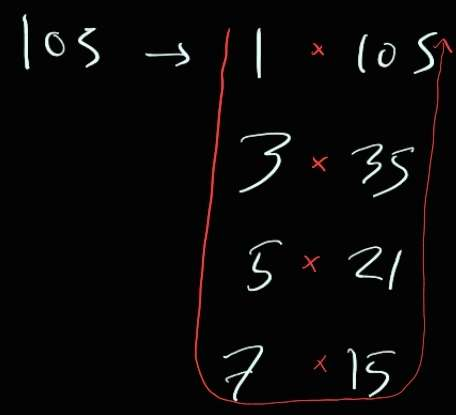
\includegraphics[scale=0.3]{sc_kotak}
\centering
\end{figure}

 Disitu aku menyadari bahwa mungkin fakta $105 = 1 \times 105 = 3 \times 35 = 5 \times 21$ bisa dipakai. Dan ya, karena dari sifat $1 < 3 < 5 < 7 < 15 < 21 < 35 < 105$ yang sesuai dengan sifat $d_1 < \dots < d_k$. Hal ini menuntunku ke fakta $d_{i} \times d_{k+1-i}=n$.


\subsection{Menggunakan $d_i \mid d_{i+1} + d_{i+2}$}
Oke, sebenarnya ini yang menurutku pribadi paling \textit{tricky}. Gimana cara menghubungkan fakta-fakta sebelumnya dengan $d_i \mid d_{i+1} + d_{i+2}$? Tentu saja kalau $i=1$ trvial, karena $1 \mid d_2+d_3$. Nah, bagaimana dengan yang lain? karena di soal sudah diberitahu secara langsung bahwa $d_k=n$ mari dicoba. Oke... $d_{k-2} \mid d_{k-1} + n$, lalu? 

\subsection{Menyadari $d_i \mid n$}
Karena setiap $d_i$ adalah pembagi dari $n$, maka $d_{k-2} \mid n$. Berarti $d_{k-2} \mid d_{k-1} + n \implies d_{k-2} \mid d_{k-1}$. Dapat $d_{k-2} \mid d_{k-1} \mid d_k$. Hmmm, sepertinya akan terbentuk keterbagian yang berbentuk \textit{chain}? Dari percobaan di awal juga (dimana $n=p^t$), jangan-jangan memang benar nanti $d_1 \mid d_2 \mid \dots \mid d_{k-2} \mid d_{k-1} \mid d_k$ karena sesuai dengan pola $d_1 = 1$, $d_2=p$, $d_3=p^2$,\dots, $d_k=p^t$.

\subsection{Menggunakan $d_{i} \times d_{k+1-i}=n$ untuk menemukan chain $d_1 \mid d_2 \mid \dots \mid d_{k-2} \mid d_{k-1} \mid d_k$}
Karena tadi aku sudah dapat fakta $d_{i} \times d_{k+1-i}=n$ berarti $d_{k-2} \mid d_{k-1} \implies \dfrac{n}{d_{3}} \mid \dfrac{n}{d_{2}} \implies d_2 \mid d_3$. Kalau begitu $d_2 \mid d_3 + d_4 \implies d_2 \mid d_4 \implies \dfrac{n}{d_{k-1}} \mid \dfrac{n}{d_{k-3}} \implies d_{k-3} \mid d_{k-1}$. Ketemu! $d_{k-3} \mid d_{k-2} + d_{k-1} \implies d_{k-3} \mid d_{k-2}$. Dari sini seharusnya kalau pakai induksinya benar akan terbukti bahwa $d_1 \mid d_2 \mid \dots \mid d_{k-2} \mid d_{k-1} \mid d_k$. Dengan sedikit pembuktian lagi bahwa tidak mungkin ada faktor prima selain $p$ yang membagi $n$ kita telah membuktikan dugaan bahwa $n=p^t$. Selesai.

\section{Solusi}
Mudah dibuktikan bahwa $n = d_1 d_{k} = d_2d_{k-1} = \dots = d_k d_1$ atau $n = d_id_{k-i+1}$ untuk setiap $1 \le i \le k$ dari sifat $d_1 < d_2 < \dots d_{k-1} < d_k$. Perhatikan karena $d_i$ adalah faktor dari $d_k = n$ untuk setiap $i=1,2,\dots,k$, maka $d_{k-1} \mid d_k$ dan $d_{k-2} \mid d_k$. Oleh karena itu $d_{k-2} \mid d_{k-1} + d_k \implies d_{k-2} \mid d_{k-1}$ yang menyebabkan $\dfrac{n}{d_3} \mid \dfrac{n}{d_2} \implies d_2 \mid d_3$.

\begin{lemma*}
$d_i \mid d_{i+1}$ untuk setiap $1 \le i \le k-1$.
\begin{proof}[\textbf{Bukti.}] Akan dibuktikan pernyataan tersebut dengan induksi di $i$. Untuk $i=1$ dan $i=2$ jelas benar bahwa $d_1 = 1 \mid d_2$ dan $d_2 \mid d_3$. Asumsikan bahwa pernyataan benar untuk $i = m$ untuk $2 \le m \le k-1$, yaitu $d_m \mid d_{m+1}$. 

Karena kita punya $d_m \mid d_{m+1} \implies \dfrac{n}{d_{k-m+1}} \mid \dfrac{n}{d_{k-m}} \implies d_{k-m} \mid d_{k-m+1}$ dan  $d_{k-m} \mid d_{k-m+1} + d_{k-m+2} \implies d_{k-m}  \mid d_{k-m+2}$, maka $\dfrac{n}{d_{m+2}} \mid \dfrac{n}{d_{m+1}} \implies d_{m+1} \mid d_{m+2}$. Hal ini menunjukkan bahwa untuk $i=m+1$, pernyataan tersebut juga berlaku. 

Dengan induksi, pernyataan terbukti.
\end{proof}
\end{lemma*}

Dari lemma tersebut didapat $1 = d_1 \mid d_2 \mid \dots \mid d_{k-1} \mid d_k = n$ yang mengakibatkan $d_i \mid d_j$ untuk setiap $1 \le i < j \le k$. Misalkan $p$ adalah faktor prima terkecil dari $n$. Akan ditunjukkan bahwa faktor prima pembagi $n$ hanyalah $p$ saja. Andaikan ada faktor prima $q > p$ dari $n$. Maka ada suatu indeks $2 \le t \le k$ sehingga $d_t = q$. Namun, dikarenakan $p$ adalah faktor prima terkecil dari $n$, maka jelas bahwa $d_2 = p$. Oleh karena $p < q$ dan $2 \le t$ maka $d_2 \mid d_t \implies p \mid q$. Kontradiksi. 

Berarti dapat disimpulkan bahwa $n$ hanya memiliki satu faktor prima saja sehingga dapat ditulis $n = p^r$ untuk suatu bilangan asli $r \ge 2$. \qed

\end{document}
